\section{Methodology}

    In this section, we described how to apply \DIFdelbegin \DIFdel{the }\DIFdelend \gls{ML} methods to design a reactor core. We followed a \DIFaddbegin \DIFadd{strict }\DIFaddend methodology consisting of three separate phases: (1) database generation, (2) machine learning, and (3) design optimization. For this, we developed a Python tool, called Plankton. The Plankton produces training and \DIFdelbegin \DIFdel{testing }\DIFdelend \DIFaddbegin \DIFadd{test }\DIFaddend datasets for given feature parameters, \DIFdelbegin \DIFdel{determines a }%DIFDELCMD < \gls{ML} %%%
\DIFdel{method based on }\DIFdelend \DIFaddbegin \DIFadd{qualifies a best-performing method among the selected }\gls{ML} \DIFadd{methods based on their }\DIFaddend performance scores, trains a predictive model for the \DIFdelbegin \DIFdel{selected }%DIFDELCMD < \gls{ML} %%%
\DIFdelend method, predicts performance metrics of designs\DIFaddbegin \DIFadd{, }\DIFaddend and finds optimal designs. The tool calls a reactor physics code to compute the performance metrics \DIFdelbegin \DIFdel{, }\DIFdelend \DIFaddbegin \DIFadd{in the database generation phase and }\DIFaddend applies an optimization technique to reveal \DIFdelbegin \DIFdel{the optimum
designs and, }\DIFdelend \DIFaddbegin \DIFadd{optimal designs in the optimization phase. It }\DIFaddend uses utilities from the scikit-learn tool \DIFdelbegin \DIFdel{for the
}\DIFdelend \DIFaddbegin \DIFadd{\mbox{%DIFAUXCMD
\cite{Ped2011} }\hspace{0pt}%DIFAUXCMD
for }\DIFaddend regression/classification\DIFdelbegin \DIFdel{analyses, }\DIFdelend \DIFaddbegin \DIFadd{, preprocessing, postprocessing, and }\DIFaddend the quantification of \DIFdelbegin \DIFdel{the quality of
predictions, preprocessing and postprocessing}\DIFdelend \DIFaddbegin \DIFadd{predictions' quality}\DIFaddend . A computational flow chart showing the main computing steps of the Plankton code is displayed in Figure~\ref{fig:flowchart}\DIFdelbegin \DIFdel{, and the computational steps are detailed in the
following sections}\DIFdelend \DIFaddbegin \DIFadd{. The following sections describe computational steps in detail}\DIFaddend .

    \begin{figure}[ht!]
    	\centering
    	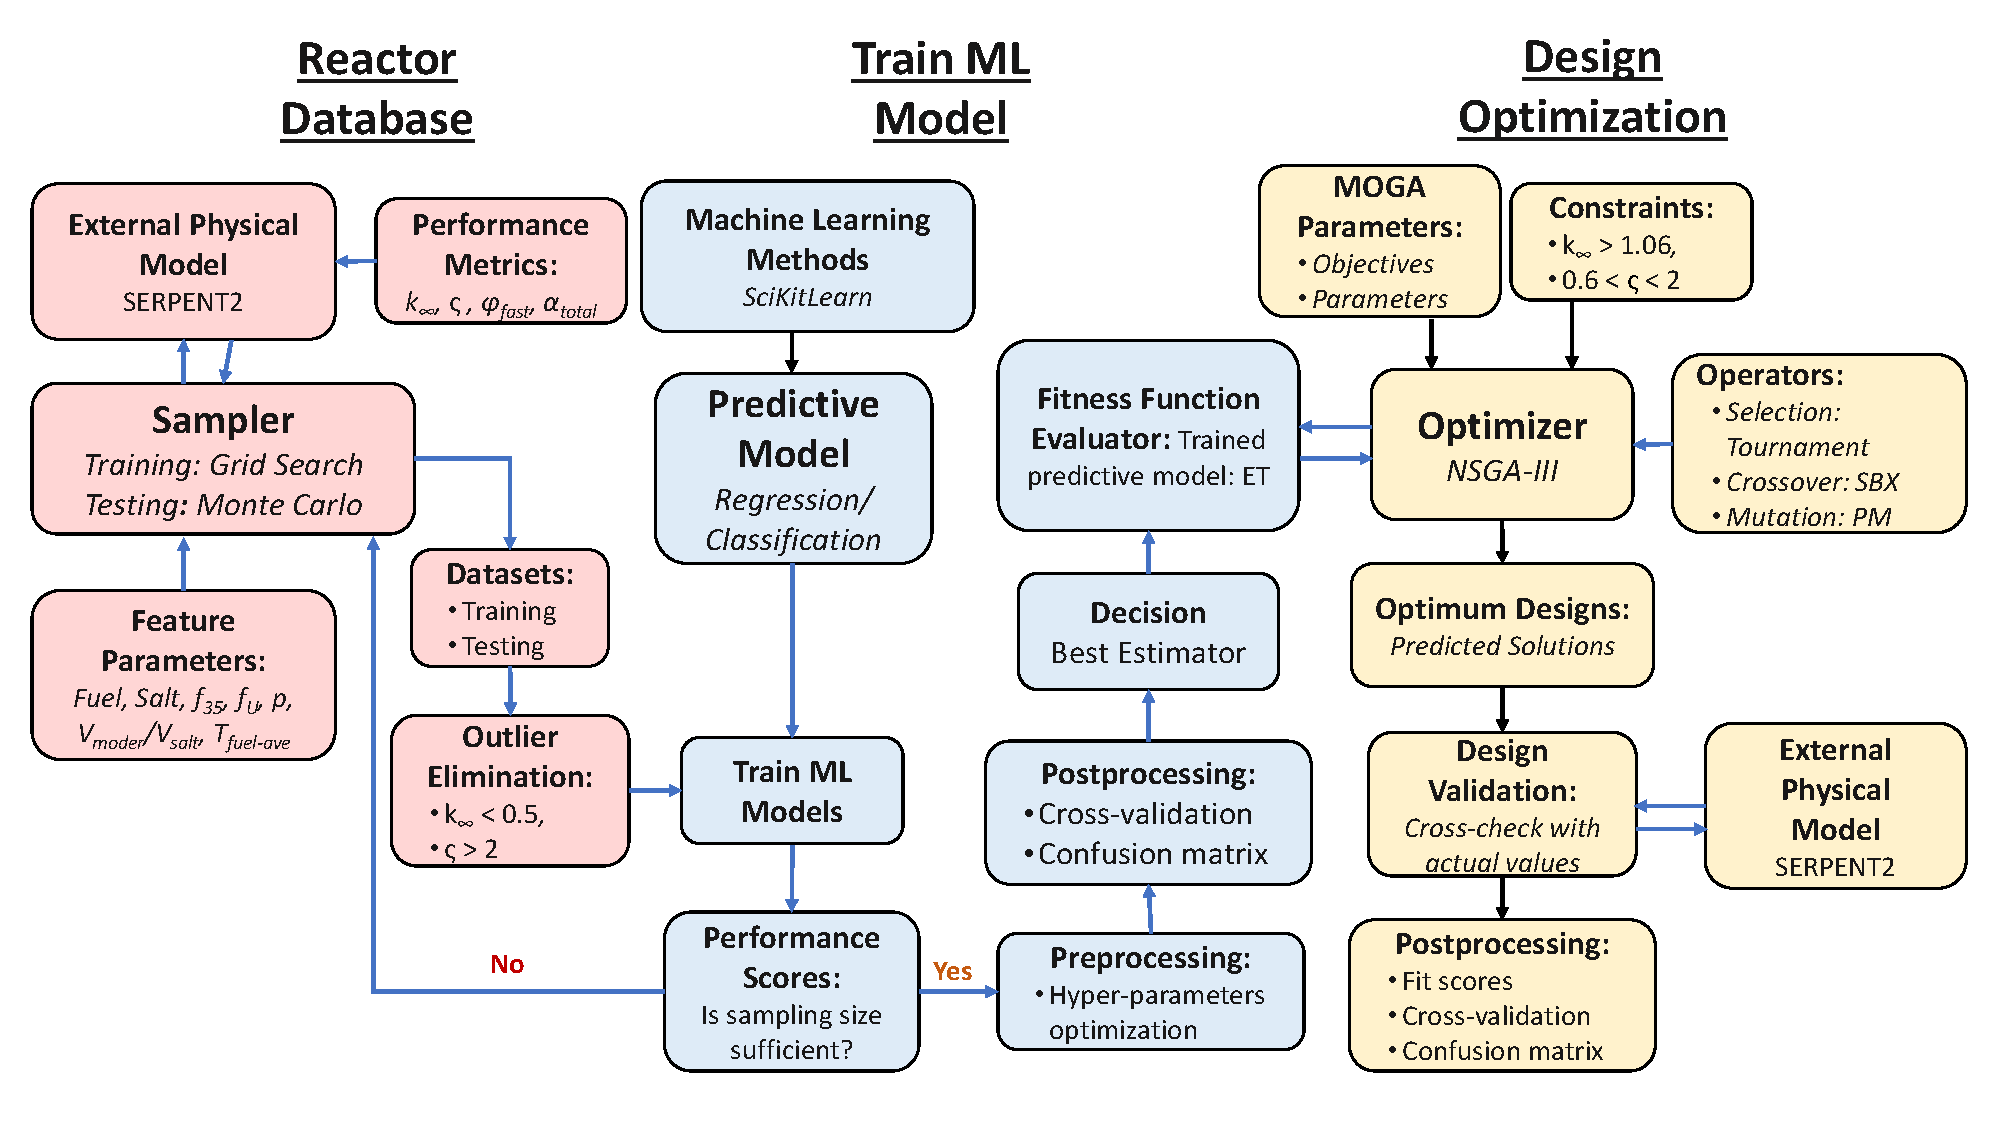
\includegraphics[trim = 0 20 0 20, clip,
    	width=\textwidth]{images/computational_flowchart.pdf}
    	\caption{Computational flowchart of the Plankton code}
    	\label{fig:flowchart}
    \end{figure}

\subsection{Plankton}

\subsubsection{Database Generation}

    \DIFdelbegin \DIFdel{The database generation is the }\DIFdelend \DIFaddbegin \DIFadd{Database generation is a }\DIFaddend step in which samplings in datasets are created and, training and \DIFdelbegin \DIFdel{testing }\DIFdelend \DIFaddbegin \DIFadd{test }\DIFaddend datasets are produced based on two distinctive sampling \DIFdelbegin \DIFdel{strategy}\DIFdelend \DIFaddbegin \DIFadd{strategies}\DIFaddend , Grid sampling and Monte Carlo.

    The grid sampling strategy, the simplest exploration approach to explore an uncertain domain, was used to obtain the training dataset. It constructs an N-dimensional grid in which each dimension accounts for a single feature parameter. \DIFaddbegin \DIFadd{Also, each dimension is discretized with the step values (the rightmost column in Table 3) into equally-spaced intervals between its upper and lower bounds. }\DIFaddend A sample in \DIFdelbegin \DIFdel{the dataset represents }\DIFdelend \DIFaddbegin \DIFadd{a dataset is represented by }\DIFaddend a specific node in the grid \DIFaddbegin \DIFadd{system}\DIFaddend .

    \DIFdelbegin \DIFdel{In contrast to }\DIFdelend \DIFaddbegin \DIFadd{Unlike }\DIFaddend the grid strategy, \DIFdelbegin \DIFdel{a }\DIFdelend \DIFaddbegin \DIFadd{the }\DIFaddend test dataset was generated by the Monte Carlo technique\DIFdelbegin \DIFdel{in which }\DIFdelend \DIFaddbegin \DIFadd{, where }\DIFaddend the value of each variable is randomly determined between \DIFdelbegin \DIFdel{the }\DIFdelend \DIFaddbegin \DIFadd{its }\DIFaddend lower and upper limits.
\DIFaddbegin 

    \DIFaddend As the size of \DIFdelbegin \DIFdel{samplings }\DIFdelend \DIFaddbegin \DIFadd{the training dataset }\DIFaddend has a significant effect on \DIFdelbegin \DIFdel{fitting scoresof the training data, the determination }\DIFdelend \DIFaddbegin \DIFadd{performance scores, the }\DIFaddend criteria for the \DIFdelbegin \DIFdel{size of datasets were explicitly defined in }\DIFdelend \DIFaddbegin \DIFadd{required size were discussed in detail in }\DIFaddend the learning curve section. \DIFdelbegin \DIFdel{Therefore, the estimation of the optimum training sample size is performed by
the ' learning $\_$curve' tool }\DIFdelend \DIFaddbegin \DIFadd{For this, we examined estimators' learning curves }\DIFaddend in conjunction with \DIFdelbegin \DIFdel{'ShuffleSplit'}\DIFdelend \DIFaddbegin \DIFadd{the cross-validation splitting strategy}\DIFaddend , which examines the change in the validation and training score of an estimator for which the number of training samples varies.

    Computational steps \DIFdelbegin \DIFdel{performed in }\DIFdelend \DIFaddbegin \DIFadd{followed in the }\DIFaddend database generation phase \DIFaddbegin \DIFadd{are as follows}\DIFaddend :
    \begin{itemize}
        \item Initialize \DIFdelbegin \DIFdel{the }\DIFdelend feature parameters, properties of which are given in Table~\ref{table:features}, for the grid search technique and Monte Carlo method.
        \item Prepare \DIFdelbegin \DIFdel{the }\DIFdelend input files for the reactor physics code for neutron transport calculation and simulate each sample in \DIFdelbegin \DIFdel{training and testing }\DIFdelend \DIFaddbegin \DIFadd{the training and test }\DIFaddend datasets.
        \item Calculate \DIFdelbegin \DIFdel{the }\DIFdelend performance metrics and extract them from the code output.
        \item Supply the prepared reactor database, a set of training/\DIFdelbegin \DIFdel{testing samples which }\DIFdelend \DIFaddbegin \DIFadd{test samples that }\DIFaddend comprise the feature parameters with \DIFaddbegin \DIFadd{the }\DIFaddend corresponding performance metrics, to the machine learning phase.
    \end{itemize}

\subsubsection{Machine Learning}

    In this part, we \DIFaddbegin \DIFadd{employed regression analysis for the estimation of performance metrics and considered classification analysis, which differs from the regression part in terms of feature parameters, to determine classes of a design. We intended to separately use both methods within the scope of this study, but we are also planning to integrate them for the determination of optimal designs for future work. We }\DIFaddend scoped out various regressors and classifiers from \gls{ML} methods \DIFdelbegin \DIFdel{with }\DIFdelend \DIFaddbegin \DIFadd{within }\DIFaddend the scikit-learn python package \cite{Ped2011} \DIFaddbegin \DIFadd{in order for the assessment of the best performing estimator(s)}\DIFaddend . Table~\ref{table:AImethods} lists \DIFaddbegin \DIFadd{the }\DIFaddend \gls{ML} methods including semi-supervised and supervised methods such as \gls{NN}, ensemble, linear, \gls{SVM}, \DIFdelbegin \DIFdel{decision tree, naive bayes, and neighbor-based }\DIFdelend \DIFaddbegin \gls{DTs}\DIFadd{, }\gls{NB}\DIFadd{, and nearest neighbours }\DIFaddend methods. Because there is more than one performance metric, \DIFdelbegin \DIFdel{the estimators need }\DIFdelend \DIFaddbegin \DIFadd{estimators require }\DIFaddend a built-in or external multi-class/multi-label support. We\DIFdelbegin \DIFdel{therefore }\DIFdelend \DIFaddbegin \DIFadd{, therefore, }\DIFaddend used the multi-target multi-output method in regression and multi-label multi-output method in classification when necessary. \DIFdelbegin \DIFdel{In this context, either 'MultiOutput' or 'OneVsRest' tools (e.g., for
}%DIFDELCMD < \gls{SV} %%%
\DIFdel{classifier) were utilized. }\DIFdelend We performed a comprehensive performance assessment by examining various regression and classification metrics given in Table~\ref{table:MLmetrics}. Prior to regression/classification analyses, we standardized our datasets by \DIFdelbegin \DIFdel{the MinMaxScaler scaler that scales }\DIFdelend \DIFaddbegin \DIFadd{scaling }\DIFaddend each feature parameter between zero and one.

    \DIFdelbegin \DIFdel{For the optimization of the hyper-parameters of the }\DIFdelend \DIFaddbegin \DIFadd{We evaluated the performances of regressors by cross-validation plots and   the performance of classifiers by confusion matrices. Cross-validation is for the visualization of prediction errors whereas confusion matrix is a table that contains all the defined classes in both the horizontal and vertical directions. In a confusion matrix, predicted outputs are listed along the top of a table whereas actual values are listed on the left-hand side column of the table. Anything on the primary diagonal is correctly predicted values. Values above and below the primary diagonal are incorrectly predicted labels called false negative and false possitive.
}

    \DIFadd{For the optimization of hyperparameters of }\DIFaddend estimators, we performed an    exhaustive search over specified parameter values \DIFdelbegin \DIFdel{using GridSearchCV within the
scikit-learn module }\DIFdelend to further improve the scores of estimators. \DIFaddbegin \DIFadd{The scoring parameters were set to f1 samples in classification and }\gls{R2} \DIFadd{in regression.
}\DIFaddend 

    Computational steps \DIFdelbegin \DIFdel{performed in }\DIFdelend \DIFaddbegin \DIFadd{followed in the }\DIFaddend machine learning phase \DIFaddbegin \DIFadd{are as follows}\DIFaddend :
    \begin{itemize}
    	\item As a starting point, use diverse \gls{ML} methods \DIFdelbegin \DIFdel{, }\DIFdelend listed in Table~\ref{table:AImethods} \DIFdelbegin \DIFdel{, }\DIFdelend from the scikit-learn tool.
    	\item With the default settings of \DIFdelbegin \DIFdel{hyper-parameters, assess the }\DIFdelend \DIFaddbegin \DIFadd{hyperparameters, assess }\DIFaddend potential estimators to be used in training just by looking into their fit \DIFdelbegin \DIFdel{performances
	}\DIFdelend \DIFaddbegin \DIFadd{scores }\DIFaddend and exclude the worst ones from the list of the potential estimators.
    	\item Analyze \DIFdelbegin \DIFdel{the }\DIFdelend learning curves of the selected estimators to understand the optimal \DIFdelbegin \DIFdel{sample size required for a }\DIFdelend \DIFaddbegin \DIFadd{size of a training dataset required for }\DIFaddend high-quality training.
    	\item Make a \DIFdelbegin \DIFdel{hyper-parameter }\DIFdelend \DIFaddbegin \DIFadd{hyperparameter }\DIFaddend optimization for the selected estimators to further improve the \DIFdelbegin \DIFdel{estimators' scores }\DIFdelend \DIFaddbegin \DIFadd{scores of the estimators}\DIFaddend .
    	\item Eliminate \DIFdelbegin \DIFdel{the outliers for which }\DIFdelend \DIFaddbegin \DIFadd{outliers according to }\DIFaddend the performance metrics \DIFdelbegin \DIFdel{which seem
	}\DIFdelend \DIFaddbegin \DIFadd{of the estimators seemingly }\DIFaddend impracticable from the viewpoint of designing a reactor and \DIFdelbegin \DIFdel{are }\DIFdelend out of interest \DIFdelbegin \DIFdel{,
	}\DIFdelend \DIFaddbegin \DIFadd{in order }\DIFaddend to further improve the estimators' scores \DIFdelbegin \DIFdel{, focusing on only the }\DIFdelend \DIFaddbegin \DIFadd{and focus on only }\DIFaddend feasible solution domain.
    	\item Select the best estimator(s) according to \DIFdelbegin \DIFdel{their fitting scores }\DIFdelend \DIFaddbegin \DIFadd{the fit scores of the estimators}\DIFaddend .
    	\item \DIFdelbegin \DIFdel{For better understanding of }\DIFdelend \DIFaddbegin \DIFadd{To better understand }\DIFaddend the selected estimators' capability, get the final scores of the estimators, cross-validate the results of the	regressors, and draw confusion matrices of the classifiers.
    	\item Supply the best estimator(s) (along with the optimized \DIFdelbegin \DIFdel{hyper-parameters}\DIFdelend \DIFaddbegin \DIFadd{hyperparameters}\DIFaddend ) to the design optimization phase to predict the performance	metrics of \DIFdelbegin \DIFdel{the }\DIFdelend objective functions.
    \end{itemize}

%%%%%%%%%%%%%%%%%%%%%%%%%%%%%%%%%%%%%%%%
    \begin{table}[ht!]
    	\centering
    	\caption{Examined \gls{ML} methods \cite{Ped2011}}
    	\begin{tabular}{ll}
    		\hline
    		\textbf{Method} & \textbf{Estimator}    \\ \hline
    		\DIFdelbeginFL \DIFdelFL{Ensemble  }\DIFdelendFL \DIFaddbeginFL \DIFaddFL{ensemble  }\DIFaddendFL & \gls{RF}, \DIFdelbeginFL \DIFdelFL{Bagging (B)  }\DIFdelendFL \DIFaddbeginFL \gls{B}  \DIFaddendFL \\
    		& \DIFdelbeginFL \DIFdelFL{AdaBoost (AB)}\DIFdelendFL \DIFaddbeginFL \gls{AB}\DIFaddendFL , \gls{ET} \\
    		& \DIFdelbeginFL \DIFdelFL{GradientBoosting (GB)   }\DIFdelendFL \DIFaddbeginFL \gls{GB}   \DIFaddendFL \\
    		\DIFdelbeginFL \DIFdelFL{Linear    }\DIFdelendFL \DIFaddbeginFL \DIFaddFL{linear    }\DIFaddendFL &\DIFdelbeginFL \DIFdelFL{ElasticNet (EN), Perceptron (P), Ridge (R) }\DIFdelendFL \DIFaddbeginFL \gls{EN}\DIFaddFL{, }\gls{P}\DIFaddFL{, }\gls{R} \DIFaddendFL \\
    		& \DIFdelbeginFL \DIFdelFL{StochasticGradientDescent (SGD)  }\DIFdelendFL \DIFaddbeginFL \gls{SGD}  \DIFaddendFL \\
    		& \DIFdelbeginFL \DIFdelFL{Lasso (L), LassoLars (LL), Logistic (Log) }\DIFdelendFL \DIFaddbeginFL \gls{L}\DIFaddFL{, }\gls{LL}\DIFaddFL{, }\gls{Log} \DIFaddendFL \\
    		\DIFdelbeginFL \DIFdelFL{Naive Bayes     }\DIFdelendFL \DIFaddbeginFL \gls{NB}  \DIFaddendFL & \DIFdelbeginFL \DIFdelFL{GaussianNB (GNB), BernoulliNB (BNB)}\DIFdelendFL \DIFaddbeginFL \gls{GNB}\DIFaddFL{, }\gls{BNB}\DIFaddendFL \\
    		\DIFdelbeginFL \DIFdelFL{Neighbor-Based  }\DIFdelendFL \DIFaddbeginFL \DIFaddFL{nearest neighbors  }\DIFaddendFL & \gls{KN} \\
    		\gls{SVM} & \DIFdelbeginFL %DIFDELCMD < \gls{SV} %%%
\DIFdelendFL \DIFaddbeginFL \gls{SVM} \DIFaddendFL \\
    		\gls{NN}  & \gls{MLP} \\
    		\DIFdelbeginFL %DIFDELCMD < \gls{DT}  %%%
\DIFdelendFL \DIFaddbeginFL \gls{DTs}  \DIFaddendFL & \gls{DT}  \\
    		\DIFdelbeginFL \DIFdelFL{Semi-Supervised }\DIFdelendFL \DIFaddbeginFL \DIFaddFL{semi-supervised }\DIFaddendFL & \DIFdelbeginFL \DIFdelFL{LabelPropagation (LP) }\DIFdelendFL \DIFaddbeginFL \gls{LP} \DIFaddendFL \\ \hline
    	\end{tabular}
    	\label{table:AImethods}
    \end{table}
    %%%%%%%%%%%%%%%%%%%%%%%%%%%%%%%%%%%%%%%%
    \begin{table}[ht!]
    	\centering
    	\caption{Metrics for \DIFaddbeginFL \DIFaddFL{the }\DIFaddendFL performance assessment of estimators \cite{Ped2011}}
    	\DIFdelbeginFL %DIFDELCMD < \resizebox{\textwidth}{!}{%
%DIFDELCMD < 		\begin{tabular}{ll}
%DIFDELCMD < 			\hline
%DIFDELCMD < 			\textbf{Regression}                  & \textbf{Classification}                  \\ \hline
%DIFDELCMD < 			fit score (fit$\_$score)             & fit score (fit$\_$score)                 \\
%DIFDELCMD < 			mean square error (MSE)              & average precision (AP)                   \\
%DIFDELCMD < 			mean absolute error (MAE)            & ranking-based average precision (LRAPS)  \\
%DIFDELCMD < 			explained variance regression (EVR)  & label ranking loss (LRL)                 \\
%DIFDELCMD < 			coefficient of determination (R$^2$) & average Hamming loss (HL)                \\
%DIFDELCMD < 			& computed area under the receiver         \\
%DIFDELCMD < 			& operating characteristic curve (ROC-AUC) \\ \hline
%DIFDELCMD < 	\end{tabular}}
%DIFDELCMD < 	%%%
\DIFdelendFL \DIFaddbeginFL \resizebox{\textwidth}{!}{%
    		\begin{tabular}{p{0.5\linewidth} p{0.5\linewidth}}
    		\hline
    		    \textbf{Regression} & \textbf{Classification} \\
    		\hline
    		    fit score: $\in$ [0, 1], best score: 1         &
                fit score: $\in$ [0, 1], best score: 1              \\
    		    \gls{MSE}, best score: 0           &
                \gls{AP}: $\in$ [0, 1], best score: 1              \\
    		    \gls{MAE}, best score: 0           &
                \gls{LRAPS}: $\in$ [0, 1], best score: 1           \\
    		    \gls{EVR}: $\in$ [0, 1], best score: 1          &
                \gls{LRL}: $\in$ [0, 1], best score: 0             \\
    		    \gls{R2}: $\in$ [0, 1], best score: 1          &
                \gls{HL}: $\in$ [0, 1], best score: 0              \\
    		  & \gls{ROCAUC}: $\in$ [0, 1], best score: 1           \\
    		\hline
    		\end{tabular}}
    	\DIFaddendFL \label{table:MLmetrics}
    \end{table}
%%%%%%%%%%%%%%%%%%%%%%%%%%%%%%%%%%%%%%%%

\subsubsection{Design Optimization}

    In the final stage of the channel design, we aimed at finding \DIFdelbegin \DIFdel{the }\DIFdelend optimal designs. We implemented a multi-variable multi-objective evolutionary algorithm \DIFaddbegin \DIFadd{appropriate to design space's structure which manifests multimodal rather than unimodal}\DIFaddend . We selected this method because optimization methods such as gradient-based or non-linear least-square do not accept discrete and non-numeric variables\DIFdelbegin \DIFdel{. We
opted for an optimization method appropriate to the problem's behavior which
manifests a convex structure rather than a linear relationship.
}\DIFdelend \DIFaddbegin \DIFadd{, and do not work well in non-convex design spaces.
}\DIFaddend 

    We defined the number of generations as a convergence stopping criterion. After finding the \DIFdelbegin \DIFdel{optimum designswith Plankton's ML methods}\DIFdelend \DIFaddbegin \DIFadd{optimal designs}\DIFaddend , we rerun Serpent tool \DIFdelbegin \DIFdel{with the optimal design }\DIFdelend \DIFaddbegin \DIFadd{\mbox{%DIFAUXCMD
\cite{Lep2014} }\hspace{0pt}%DIFAUXCMD
with their }\DIFaddend feature parameters to crosscheck the solutions. \DIFdelbegin \DIFdel{Thus, we
performed additional neutron transport calculations for the optimal designs via
the reactor physics code, used to generate the reactor database. Acceptance
criteria for the }\DIFdelend \DIFaddbegin \DIFadd{The acceptance criterion for the }\DIFaddend accuracy of the optimal designs was selected as:
    \begin{eqnarray}\label{Eq0}
    \dfrac{x_{i,a}-x_{i,p}}{x_{i,a}} \leq 5%DIF < 
\DIFaddbegin \DIFadd{\%
    }\DIFaddend \end{eqnarray}
    where $x_{i,a}$ is the actual value of i$th$ metric and $x_{i,p}$ is the predicted value of i$th$ metric.

    Computational steps \DIFdelbegin \DIFdel{performed in }\DIFdelend \DIFaddbegin \DIFadd{followed in the }\DIFaddend design optimization phase \DIFaddbegin \DIFadd{are as follows}\DIFaddend :
    \begin{itemize}
    	\item \DIFdelbegin \DIFdel{Initialize the }\DIFdelend \DIFaddbegin \DIFadd{Specify an optimization tool (}\DIFaddend \gls{MOGA} \DIFdelbegin \DIFdel{parameters including }\DIFdelend \DIFaddbegin \DIFadd{method) consistent with the structure of the feature parameters and the problem at hand.
        }\item \DIFadd{Determine tool's parameters such as }\DIFaddend decision variables, operators, number of generations, \DIFaddbegin \DIFadd{and }\DIFaddend initial population size\DIFdelbegin \DIFdel{, crossover rate
	and mutation ratio}\DIFdelend .
    	\item Define \DIFdelbegin \DIFdel{the }\DIFdelend constraints for the performance metrics \DIFdelbegin \DIFdel{which would
	}\DIFdelend \DIFaddbegin \DIFadd{to }\DIFaddend eliminate undesired designs.
    	\item \DIFdelbegin \DIFdel{Use a }%DIFDELCMD < \gls{GA} %%%
\DIFdel{method, which are naturally
	limited by the problem, consistent with the structure of the feature parameters.
	}%DIFDELCMD < \item %%%
\item%DIFAUXCMD
\DIFdel{Couple the estimator (s) to the }%DIFDELCMD < \gls{GA} %%%
\DIFdel{method to calculate the
	}\DIFdelend \DIFaddbegin \DIFadd{Integrate the optimizer with the best performing estimator (in place of reactor physics code) to evaluate the }\DIFaddend performance metrics of \DIFdelbegin \DIFdel{the objective functions, without running a reactor physics
	code}\DIFdelend \DIFaddbegin \DIFadd{objective functions}\DIFaddend .
    	\item Iterate this \gls{ML}-\gls{GA} coupled system until either the constraints are met or the solutions are converged to one of the predefined criteria.
    	\item \DIFdelbegin \DIFdel{Verify the pareto-front }\DIFdelend \DIFaddbegin \DIFadd{Validate Pareto-front }\DIFaddend (predicted) solutions \DIFdelbegin \DIFdel{by calculating actual values }\DIFdelend \DIFaddbegin \DIFadd{with actual values (with additional Serpent simulation)}\DIFaddend .
    \end{itemize}

\subsection{Channel Design with Plankton}

\subsubsection{Design Parameters}

    We applied the suggested method to a single fuel channel \gls{MSR} geometry with square unit cell approximation to use in a basic geometry with the least number of feature parameters and performance metrics. An illustration of the channel geometry is shown in Figure~\ref{fig:channel}. \DIFaddbegin \DIFadd{In the figure, $p$ is the pitch length, $T_{in}$ and $T_{out}$ are inlet and outlet temperatures, $v_{salt}$ is the velocity of fuel-salt, $L$ is the channel length, $R_f$ is the radius of the fuel-salt channel and $q_{channel}$ is the total heat generation in the channel. }\DIFaddend Feature parameters describing \DIFdelbegin \DIFdel{the
}\DIFdelend material and geometry properties of the \DIFdelbegin \DIFdel{single }\DIFdelend channel were selected as fuel type, salt type, $^{235}$U fraction ($f_{35}$) in U, U fraction ($f_{U}$) in heavy metal, channel-to-channel pitch length ($p$), moderator-to-salt volume ratio ($\xi$), and average fuel-salt temperature ($T_{ave}$) along the channel. We varied \DIFdelbegin \DIFdel{the }\DIFdelend \DIFaddbegin \DIFadd{these }\DIFaddend variables between upper and lower bounds described in Table~\ref{table:features}. The $^{235}$U fraction in U was limited to 20 wt.\% which is the maximum limit for \gls{HALEU}. For the fuel types other than U fuel type, U content in heavy metal varies from 10 to 90 wt.\%. The maximum $p$, based on \gls{ORNL}'s \gls{MSRE} design \DIFaddbegin \DIFadd{\mbox{%DIFAUXCMD
\cite{robertson1971}}\hspace{0pt}%DIFAUXCMD
}\DIFaddend , was set to 16 cm. \DIFdelbegin \DIFdel{The $\xi$ variable
was calculated from }\DIFdelend \DIFaddbegin \DIFadd{From }\DIFaddend the ratio of pitch \DIFdelbegin \DIFdel{to fuel salt radius between }\DIFdelend \DIFaddbegin \DIFadd{length to fuel-salt channel radius ($p/R_{f}$), the $\xi$ variable was calculated and found in the range of }\DIFaddend 0.274 (\DIFdelbegin \DIFdel{p/D$_{fuel}$ }\DIFdelend \DIFaddbegin \DIFadd{$p/R_{f}$ }\DIFaddend = \DIFdelbegin \DIFdel{1}\DIFdelend \DIFaddbegin \DIFadd{0.5}\DIFaddend ) and 10.46 (\DIFdelbegin \DIFdel{p/D$_{fuel}$ }\DIFdelend \DIFaddbegin \DIFadd{$p/R_{f}$ }\DIFaddend = \DIFdelbegin \DIFdel{3}\DIFdelend \DIFaddbegin \DIFadd{1.5}\DIFaddend ).

    We studied three different fuel types, U, U-Th\DIFaddbegin \DIFadd{, }\DIFaddend and U-Pu in this work. Th in U-Th contains only $^{232}$Th isotope whereas Pu in U-Pu comes from the \DIFdelbegin \DIFdel{weapon-grade
}\DIFdelend \DIFaddbegin \DIFadd{weapons-grade }\DIFaddend Pu constituting the following isotopes: $^{238}$Pu (0.05 at.\%), $^{239}$Pu (94.3 at.\%), $^{240}$Pu (5 at.\%), $^{241}$Pu (0.6 at.\%) and $^{242}$Pu (0.05 at.\%). It is assumed that there is no $^{234}$U in U as a parasitic absorber.

    We examined three types of different salts widely used in prototype reactors by various companies (Terrestrial Energy, Terrapower, Thorcon, etc.): LiF-BeF$_2$, NaF-BeF$_2$, and NaCl. The upper value of \DIFaddbegin \DIFadd{the }\DIFaddend average fuel-salt temperature ($T_{ave}$) is set to 1200 K while its base temperature used to calculate the total feedback coefficient of reactivity is 900 K. As the temperature is the main driver for \DIFdelbegin \DIFdel{fuel salt }\DIFdelend \DIFaddbegin \DIFadd{fuel-salt }\DIFaddend density and Doppler effect \DIFdelbegin \DIFdel{on }\DIFdelend \DIFaddbegin \DIFadd{of }\DIFaddend feedback, salt density variation with the $T_{ave}$ was taken into account based on the reports \cite{Janz1988, Jerden2019}.

    \DIFdelbegin \DIFdel{The }\DIFdelend \DIFaddbegin \DIFadd{In the regression analysis, the }\DIFaddend most critical performance metrics are \DIFdelbegin \DIFdel{the }\DIFdelend \DIFaddbegin \DIFadd{selected as }\DIFaddend infinite multiplication factor ($k_{\infty}$), conversion ratio ($\varsigma$), fast flux ($\phi_{fast}$) incident on the graphite moderator\DIFaddbegin \DIFadd{, }\DIFaddend and total feedback coefficient (${\alpha_{total}}$). \DIFdelbegin \DIFdel{However, ${\alpha_{total}}$ was not considered as performance metrics in ML phase as it can be calculated }\DIFdelend \DIFaddbegin \DIFadd{But, we did not include the ${\alpha_{total}}$ as a performance metric since this metric caused huge errors in scores, probably due to zero values at 900 K. Yet, we }\DIFaddend promptly and accurately \DIFaddbegin \DIFadd{calculated it }\DIFaddend from Eq. \protect\ref{Eq1} using $k_{\infty}$ \DIFdelbegin \DIFdel{, thus being calculated }\DIFdelend at the end of the design optimization phase.

    In \DIFaddbegin \DIFadd{the }\DIFaddend classification analysis, \DIFdelbegin \DIFdel{a channel design was labeled }\DIFdelend \DIFaddbegin \DIFadd{the ${\alpha_{total}}$ metric did not cause any trouble so that we were able to use it. We labeled the single channel design }\DIFaddend with different labels according to its spectrum, type, criticality condition\DIFaddbegin \DIFadd{, }\DIFaddend and positive or \DIFaddbegin \DIFadd{the }\DIFaddend negative sign of the feedback coefficient. Accordingly, we addressed any channel design as breeder type when $\varsigma \geq 1.0$, as fast spectrum when \gls{EALF} $\geq 1eV$, as supercritical condition when $k_{\infty} \geq 1.0$, and as positive feedback when ${\alpha_{total}} \geq 0.0$. For the opposite of these conditions, the design is labeled as burner type, thermal spectrum, sub-critical condition, and negative feedback, respectively.

    Associated with the channel design, we made the following approximations, simplifications\DIFaddbegin \DIFadd{, }\DIFaddend and approaches involved in the model/method development:
    \begin{itemize}
    	\item The unit cell approximation \DIFdelbegin \DIFdel{with }\DIFdelend \DIFaddbegin \DIFadd{in }\DIFaddend a square lattice \DIFaddbegin \DIFadd{geometry }\DIFaddend was chosen to represent the single channel geometry. It is an effective geometry structure for periodicity.
    	\item The fuel-salt \DIFdelbegin \DIFdel{is }\DIFdelend \DIFaddbegin \DIFadd{was }\DIFaddend assumed to be stationary, by neglecting thermal-hydraulic effects such as delayed neutron precursor movement.
    	\item Calculations were performed for initial fuel loading assuming fresh fuel.
    	\item \DIFdelbegin \DIFdel{Total }\DIFdelend \DIFaddbegin \DIFadd{The total }\DIFaddend heat generation	rate along the channel \DIFdelbegin \DIFdel{is }\DIFdelend \DIFaddbegin \DIFadd{was }\DIFaddend expressed in terms of an arithmetic average of the inlet and outlet temperatures, i.e., $T_{ave}$ = ($T_{in}$+$T_{out}$)/2, thereby \DIFdelbegin \DIFdel{, }\DIFdelend making the design independent from the length	of the channel.
    \end{itemize}

    Using these approximations, we eliminated four interdependent variables: inlet and outlet temperatures, heat generation rate, and channel length\DIFdelbegin \DIFdel{, to the
average temperature definition}\DIFdelend . We reduced the total number of feature parameters from eleven to seven parameters.

%%%%%%%%%%%%%%%%%%%%%%%%%%%%%%%%%%%%%%%%
    \begin{figure}[ht!]
    	\centering
    	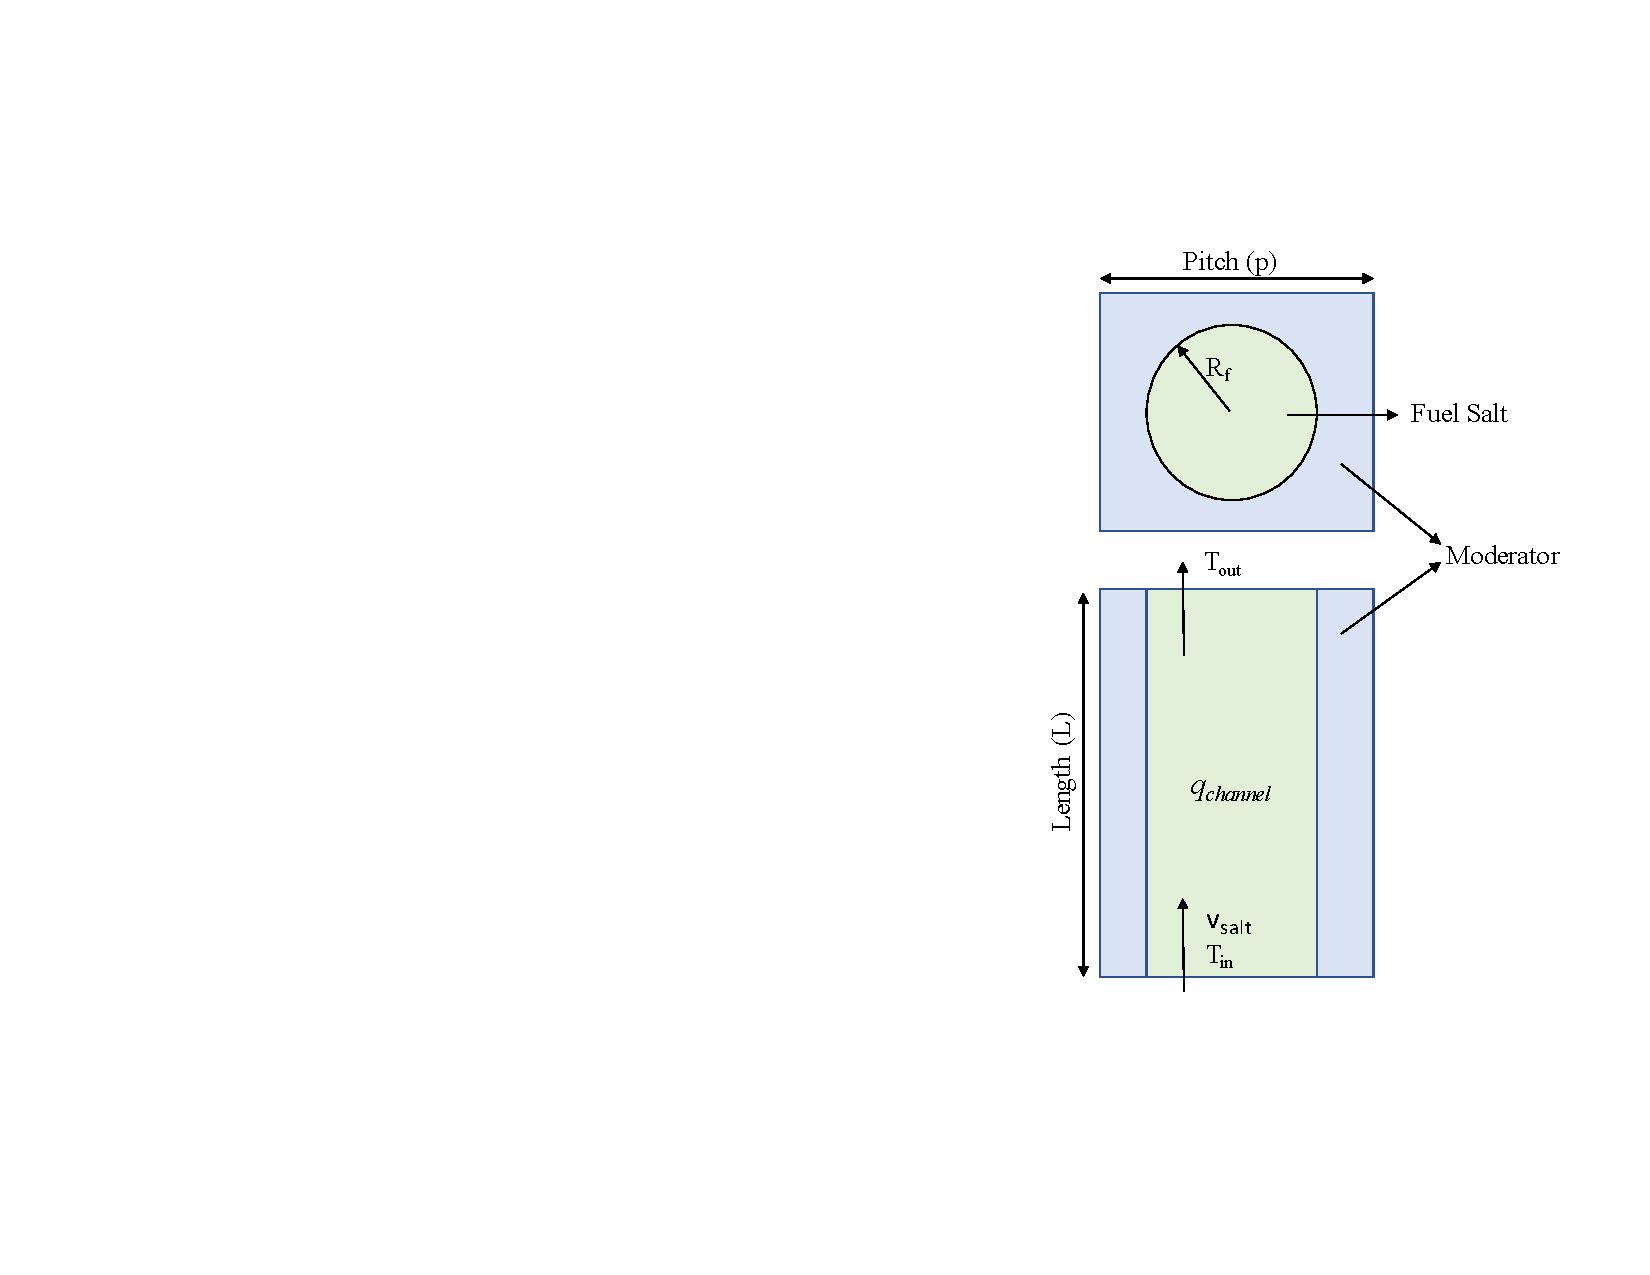
\includegraphics[trim=500 140 0 100, clip,
    	scale=0.6]{images/single_channel.pdf}
    	\caption{Single fuel channel representation\DIFaddbeginFL \DIFaddFL{.}\DIFaddendFL }
    	\label{fig:channel}
    \end{figure}
%%%%%%%%%%%%%%%%%%%%%%%%%%%%%%%%%%%%%%%%
    \begin{table}[ht!]
    	\centering
    	\caption{Feature parameters for database generation}
    	\begin{tabular}{lllll}
    		\hline
    		\textbf{Variable} & \textbf{Distribution} & \textbf{Material types} & 		& \textbf{Steps} \\ \hline
    		Fuel Type & Discrete   & U, U-Th, U-Pu & & 3 \\
    		Salt Type & Discrete   & LiF-BeF$_2$, NaCl, & NaF-BeF$_2$  & 3 \\
    		&  & \textbf{Lower value} &\textbf{Upper value} &  \\
    		$f_{35}$  & Continuous  & 1 wt.\%   & 20 wt.\% & 10 \\
    		$f_{U}$   & Continuous  & 10 wt.\%  & 90 wt.\% & 9 \\
    		$p$       & Continuous  & 1 cm      & 16 cm & 10 \\
    		$\xi$     & Continuous  & 0.274 & 10.46 & 10 \\
    		$T_{ave}$ & Continuous  & 900 K     & 1200 K & 5 \\ \hline
    	\end{tabular}
    	\label{table:features}
    \end{table}
%%%%%%%%%%%%%%%%%%%%%%%%%%%%%%%%%%%%%%%%

\subsubsection{Optimization Parameters}

    We used the \gls{NSGAIII} \cite{deb2014, jain2014} from the pymoo tool \cite{pymoo2020} as an optimizer with the \gls{SBX} and \gls{PM} operators. The population size and number of generations were set to 150 and 5000, respectively. \DIFdelbegin \DIFdel{Tournament }\DIFdelend \DIFaddbegin \DIFadd{The tournament }\DIFaddend selection, in which a set of chromosomes are selected randomly and then the fittest chromosomes are selected for further operation, was employed to select the fittest candidates from the current generation.

    Several independent constraints imposed by the basic requisites of a \gls{MSR} design were implemented to the solution objectives in \DIFdelbegin \DIFdel{accordance with the references \mbox{%DIFAUXCMD
\cite{rykhlevskii2019, betzler2017, ashraf2019} }\hspace{0pt}%DIFAUXCMD
}\DIFdelend \DIFaddbegin \DIFadd{line with the given references \mbox{%DIFAUXCMD
\cite{robertson1971, rykhlevskii2019, betzler2017, ashraf2019} }\hspace{0pt}%DIFAUXCMD
}\DIFaddend in the following way: \DIFaddbegin \DIFadd{We searched for }\DIFaddend $k_{\infty}$ \DIFdelbegin \DIFdel{is }\DIFdelend greater than 1.06 to make up for neutron leakage\DIFdelbegin \DIFdel{; }\DIFdelend \DIFaddbegin \DIFadd{. Despite the MSRs typically have a conversion ratio of around 1.0, }\DIFaddend $\varsigma$ \DIFdelbegin \DIFdel{is
}\DIFdelend \DIFaddbegin \DIFadd{was chosen as }\DIFaddend higher than 0.6 \DIFdelbegin \DIFdel{; and }\DIFdelend \DIFaddbegin \DIFadd{to include as many designs as into the optimization process. As there is no reported constraints on }\DIFaddend $\phi_{fast}$\DIFaddbegin \DIFadd{, we simply assumed $\phi_{fast}$ }\DIFaddend per source neutron on graphite \DIFdelbegin \DIFdel{in which }\DIFdelend \DIFaddbegin \DIFadd{to be lower than half (50) of what }\DIFaddend the maximum value \DIFdelbegin \DIFdel{is calculated to be about 100 is less than 50.
}\DIFdelend \DIFaddbegin \DIFadd{($\sim100$) of the fast flux in the training dataset is.
}\DIFaddend 

    \DIFdelbegin \DIFdel{In the optimizationproblem, the }\DIFdelend \DIFaddbegin \DIFadd{For optimization, }\DIFaddend feature parameters were assigned as decision variables\DIFdelbegin \DIFdel{while the }\DIFdelend \DIFaddbegin \DIFadd{, while }\DIFaddend performance metrics were assigned as solution objectives (or objective functions). The $k_{\infty}$ and $\varsigma$ metrics were maximized while the $\phi_{fast}$ was minimized.

\subsubsection{Neutronic Simulator}

    We employed a Monte Carlo neutron transport tool, Serpent 2 (2.1\DIFdelbegin \DIFdel{.30}\DIFdelend \DIFaddbegin \DIFadd{.31}\DIFaddend ) \cite{Lep2014} to compute \DIFdelbegin \DIFdel{the performance metricsdefined in design parameters
section}\DIFdelend \DIFaddbegin \DIFadd{performance metrics}\DIFaddend . It uses ENDF/B-VII.0 \cite{chadwick2006} as the neutron cross-section library \DIFdelbegin \DIFdel{along with }\DIFdelend \DIFaddbegin \DIFadd{alongside the }\DIFaddend S(${\alpha}$, ${\beta}$) thermal scattering libraries. In the simulator, neutron population per cycle, passive cycle, and active cycle were set to 2000, 50, and 100, respectively, to yield a computational standard error of less than 100 pcm in the $k_{\infty}$. A two-group neutron energy structure for the calculation of $\phi_{fast}$ on the moderator was used\DIFaddbegin \DIFadd{, }\DIFaddend and lower and upper energy boundaries for the fast region were set to 0.625 eV and 20 MeV, respectively. The $k_{\infty}$, $\varsigma$, and $\phi_{fast}$ metrics were directly extracted from the output file whereas ${\alpha_{total}}$ was calculated by Eq. \protect\ref{Eq1}:
    \begin{eqnarray}\label{Eq1}
    \alpha_{total} = \dfrac{\partial\rho}{\partial T} \approx
    \dfrac{\Delta\rho}{\Delta T}=\dfrac{\rho-\rho_b}{T-T_b}
    \end{eqnarray}
    where $\rho$ is the reactivity, $\rho_b$ is the reactivity at the base temperature, $T$ is the temperature, and $T_b$ is the base temperature. However, we purposefully avoided using $\partial \rho /\partial T$ in estimating \DIFdelbegin \DIFdel{/predicting the feedback coefficient as }\DIFdelend \DIFaddbegin \DIFadd{the }\DIFaddend ${\alpha_{total}}$ \DIFaddbegin \DIFadd{since it }\DIFaddend goes to infinity when $T_{ave}$ is very close to the base temperature\DIFdelbegin \DIFdel{, resulting
problematic outputs}\DIFdelend . Instead, we used $\partial k$(mk) and converted to ${\alpha_{total}}$ at the end of the calculations. For the \DIFdelbegin \DIFdel{energy spectrum
classification of the reactor , }\DIFdelend \DIFaddbegin \DIFadd{estimation of reactor spectrum in classification, we used }\DIFaddend the \gls{EALF}  value \DIFdelbegin \DIFdel{extracted from the output
file was used}\DIFdelend \DIFaddbegin \DIFadd{given in the code output}\DIFaddend .

\subsubsection{Datasets}
    In this work, a total training sample size of 285000 and a total test sample
    size of 8000 were used.


